\documentclass[10pt,twoside,twocolumn]{book}
\usepackage[bg-letter]{lib/rpg-book} % Options: bg-a4, bg-letter, bg-full, bg-print, bg-none.
\usepackage[english]{babel}
\usepackage[utf8]{inputenc}
\usepackage[hidelinks]{hyperref}

\usepackage[T1]{fontenc}
\usepackage{tgcursor}
\usepackage{xcolor}
\usepackage{enumitem}
\usepackage{wrapfig}
\usepackage{caption}
\usepackage{subcaption}
\usepackage{float}
\usepackage{pdfpages}

\usepackage{rotating}
\usepackage{tikz}

\makeatletter
\newcommand{\globalcolor}[1]{%
  \color{#1}\global\let\default@color\current@color
}
\makeatother

\makeatletter
\def\newsect{%
    \vskip2em plus0.5em minus0.5em%
    \hbox to\linewidth{\hfil*\quad\quad*\quad\quad*\hfil}%
    \penalty10000\vskip2em plus0.5em minus0.5em%
    \@afterindentfalse\@afterheading%
}
\makeatother%


\definecolor{alien}{rgb}{1, 1, 0.9}

\definecolor{PC}{HTML}{c0ccc1}


\newcommand\pc[1]{\colorbox{PC}{\color{black} #1}}

%  

\AtBeginDocument{\globalcolor{alien}}

\title{Untitled Cinematic Scenario}
\date{\today}
\author{Arthur Marques \\ u/marques\_art\_boris}





% Start document
\begin{document}
\fontfamily{ppl}\selectfont % Set text font
\frontmatter

\maketitle


\begin{rpg-commentbox}{Overview}
  Biohazard is a complete cinematic scenario for Alien roleplaying game. Players take the role of corporate firefighters trying to save the space station medical facility, or so they were told.

  This is a short cinematic scenario, ideal for a single session or perhaps 2 sessions where you can dive more into details and allow more openness. I estimate that the whole booklet can be finished in a 6 to 8h game (preferably 2 sessions).
\end{rpg-commentbox}



\medskip
\begin{rpg-commentbox}{A note form the author}
  \textbf{Full disclosure:} I apologize to those who put their lives at risk doing such an amazing job for any inaccuracies in this adventure. I am a humble student and my knowledge of firefighters is based on whatever I could gather/read/watch to write this adventure. 
  
  Ultimately, this is still a game with its limitations and I do hope that people have fun playing this cinematic scenario.
  \begin{flushright}
  -- Arthur Marques
  \end{flushright}
\end{rpg-commentbox}



\begin{rpg-warnbox}{Another note form the author}
  The following content contains mature situations/themes and is intended for an adult audience. The opinions expressed here do not necessarily reflect my personal opinions. Readers discretion is advised.

  Other red boxes in the booklet are often optional and explicitly have gore descriptions. Use them only if you and all players are comfortable.

  \begin{flushright}
  -- Arthur Marques
  \end{flushright}
\end{rpg-warnbox}


\makebox[0pt][l]{%
  \raisebox{-\totalheight}[-20pt][0pt]{%
    \hspace*{-0.5cm}%
    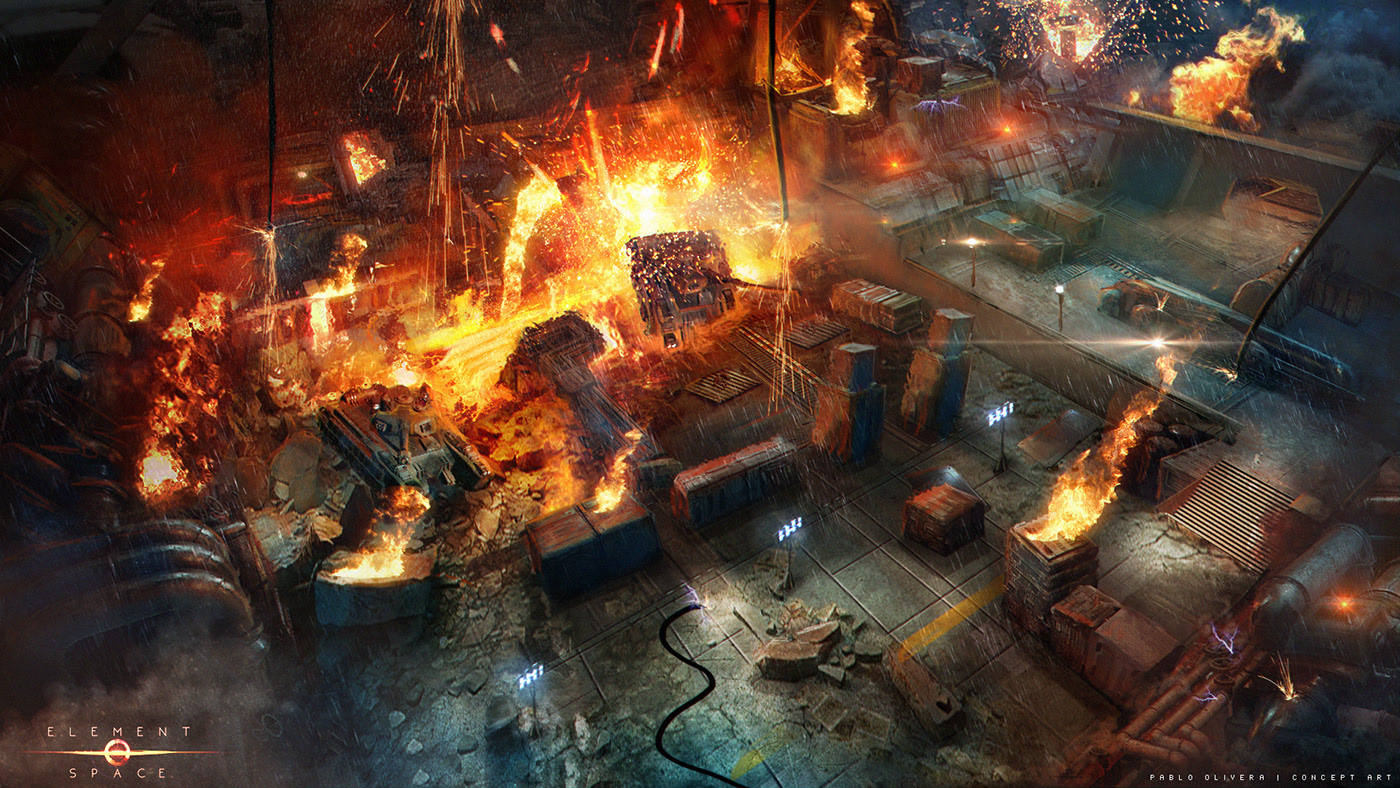
\includegraphics[width=1.0\textwidth]{img/bg/fire.jpg}}}%


\clearpage



\tableofcontents

\mainmatter

\chapter{Situation}

\begin{rpg-commentbox}{Overview}
    Melting Point is a complete cinematic scenario for Alien roleplaying game. The intention is that the scenario can be played from two different perspectives: corporate crew \& prisoners. In the current draft, I focus on prisoners.
\end{rpg-commentbox}


\section{Scenario Overview}

The setup is quite straightforward: Weyland-Yutani Kohru, lithium refinery station operates under United Americas surveillance. 
The corporation provides technical knowhow while the government provides labor force in the form of captured terrorists. 


While under a not so standard annual inspection, hell cuts lose as the station enters quarantine lock-down due to an unexpected event.
What will the station crew do? Will the prisoners ally or will old grudges turn them one against the others? 

Many of the prisioners at Kohru had never faced trial or charges, they were caught under the United America terrorist act. Lack of communication, time for lawyers to travel to the place and the edge of the charted systems, and all the corporate bureaucracy has made the location a living nightmare.  




\medskip
\begin{rpg-commentbox}{Science Background}
\begin{small}
\textit{Lithium is a highly reactive alkali metal that offers excellent heat and electrical conductivity.  These properties make it particularly useful for the manufacture of glass, high-temperature lubricants, chemicals, pharmaceuticals, and lithium ion batteries for electric cars and consumer electronics}

\textit{The process for recovering lithium from ore can vary based on the specific mineral deposit in question. In general, the process entails removing the mineral material from the earth then heating and pulverizing it. The crushed mineral powder is combined with chemical reactants, such as sulfuric acid, then the slurry is heated, filtered, and concentrated through an evaporation process to form saleable lithium carbonate, while the resulting wastewater is treated for reuse or disposal.}    
\end{small}
\end{rpg-commentbox}




The station operates on a cryosleep round robin algorithm, i.e., to avoid riots only a handful prisoners are awake at any given time. Other cryosleep chambers are heavily protected and out of limits. Prisoners awake from cryosleep and start the refinery work. 

At each round robin rotation, a synthetic is put alongside the prisoners so that it can gather data about potential terrorist attacks, evidence, and information for blackmailing purposes. One of the players agenda should be replaced by the synthetic agenda. 


Weapons and tooling at the location work either with biometric fingerprints or geo-location. For instance, a prisoner cannot light a welding torch near elevator entrances, or only security staff can fire pistols.





\medskip
\begin{rpg-commentbox}{Setting game difficulty}
\begin{itemize}
    \item \textbf{Normal}: as described in the booklet;
    \item \textbf{Hard}: non-lethal weapons only, e.g., shotguns fire rubber bullets;
\end{itemize}
\end{rpg-commentbox}

\newsect

\newpage

\begin{sidewaysfigure*}
    \centering
    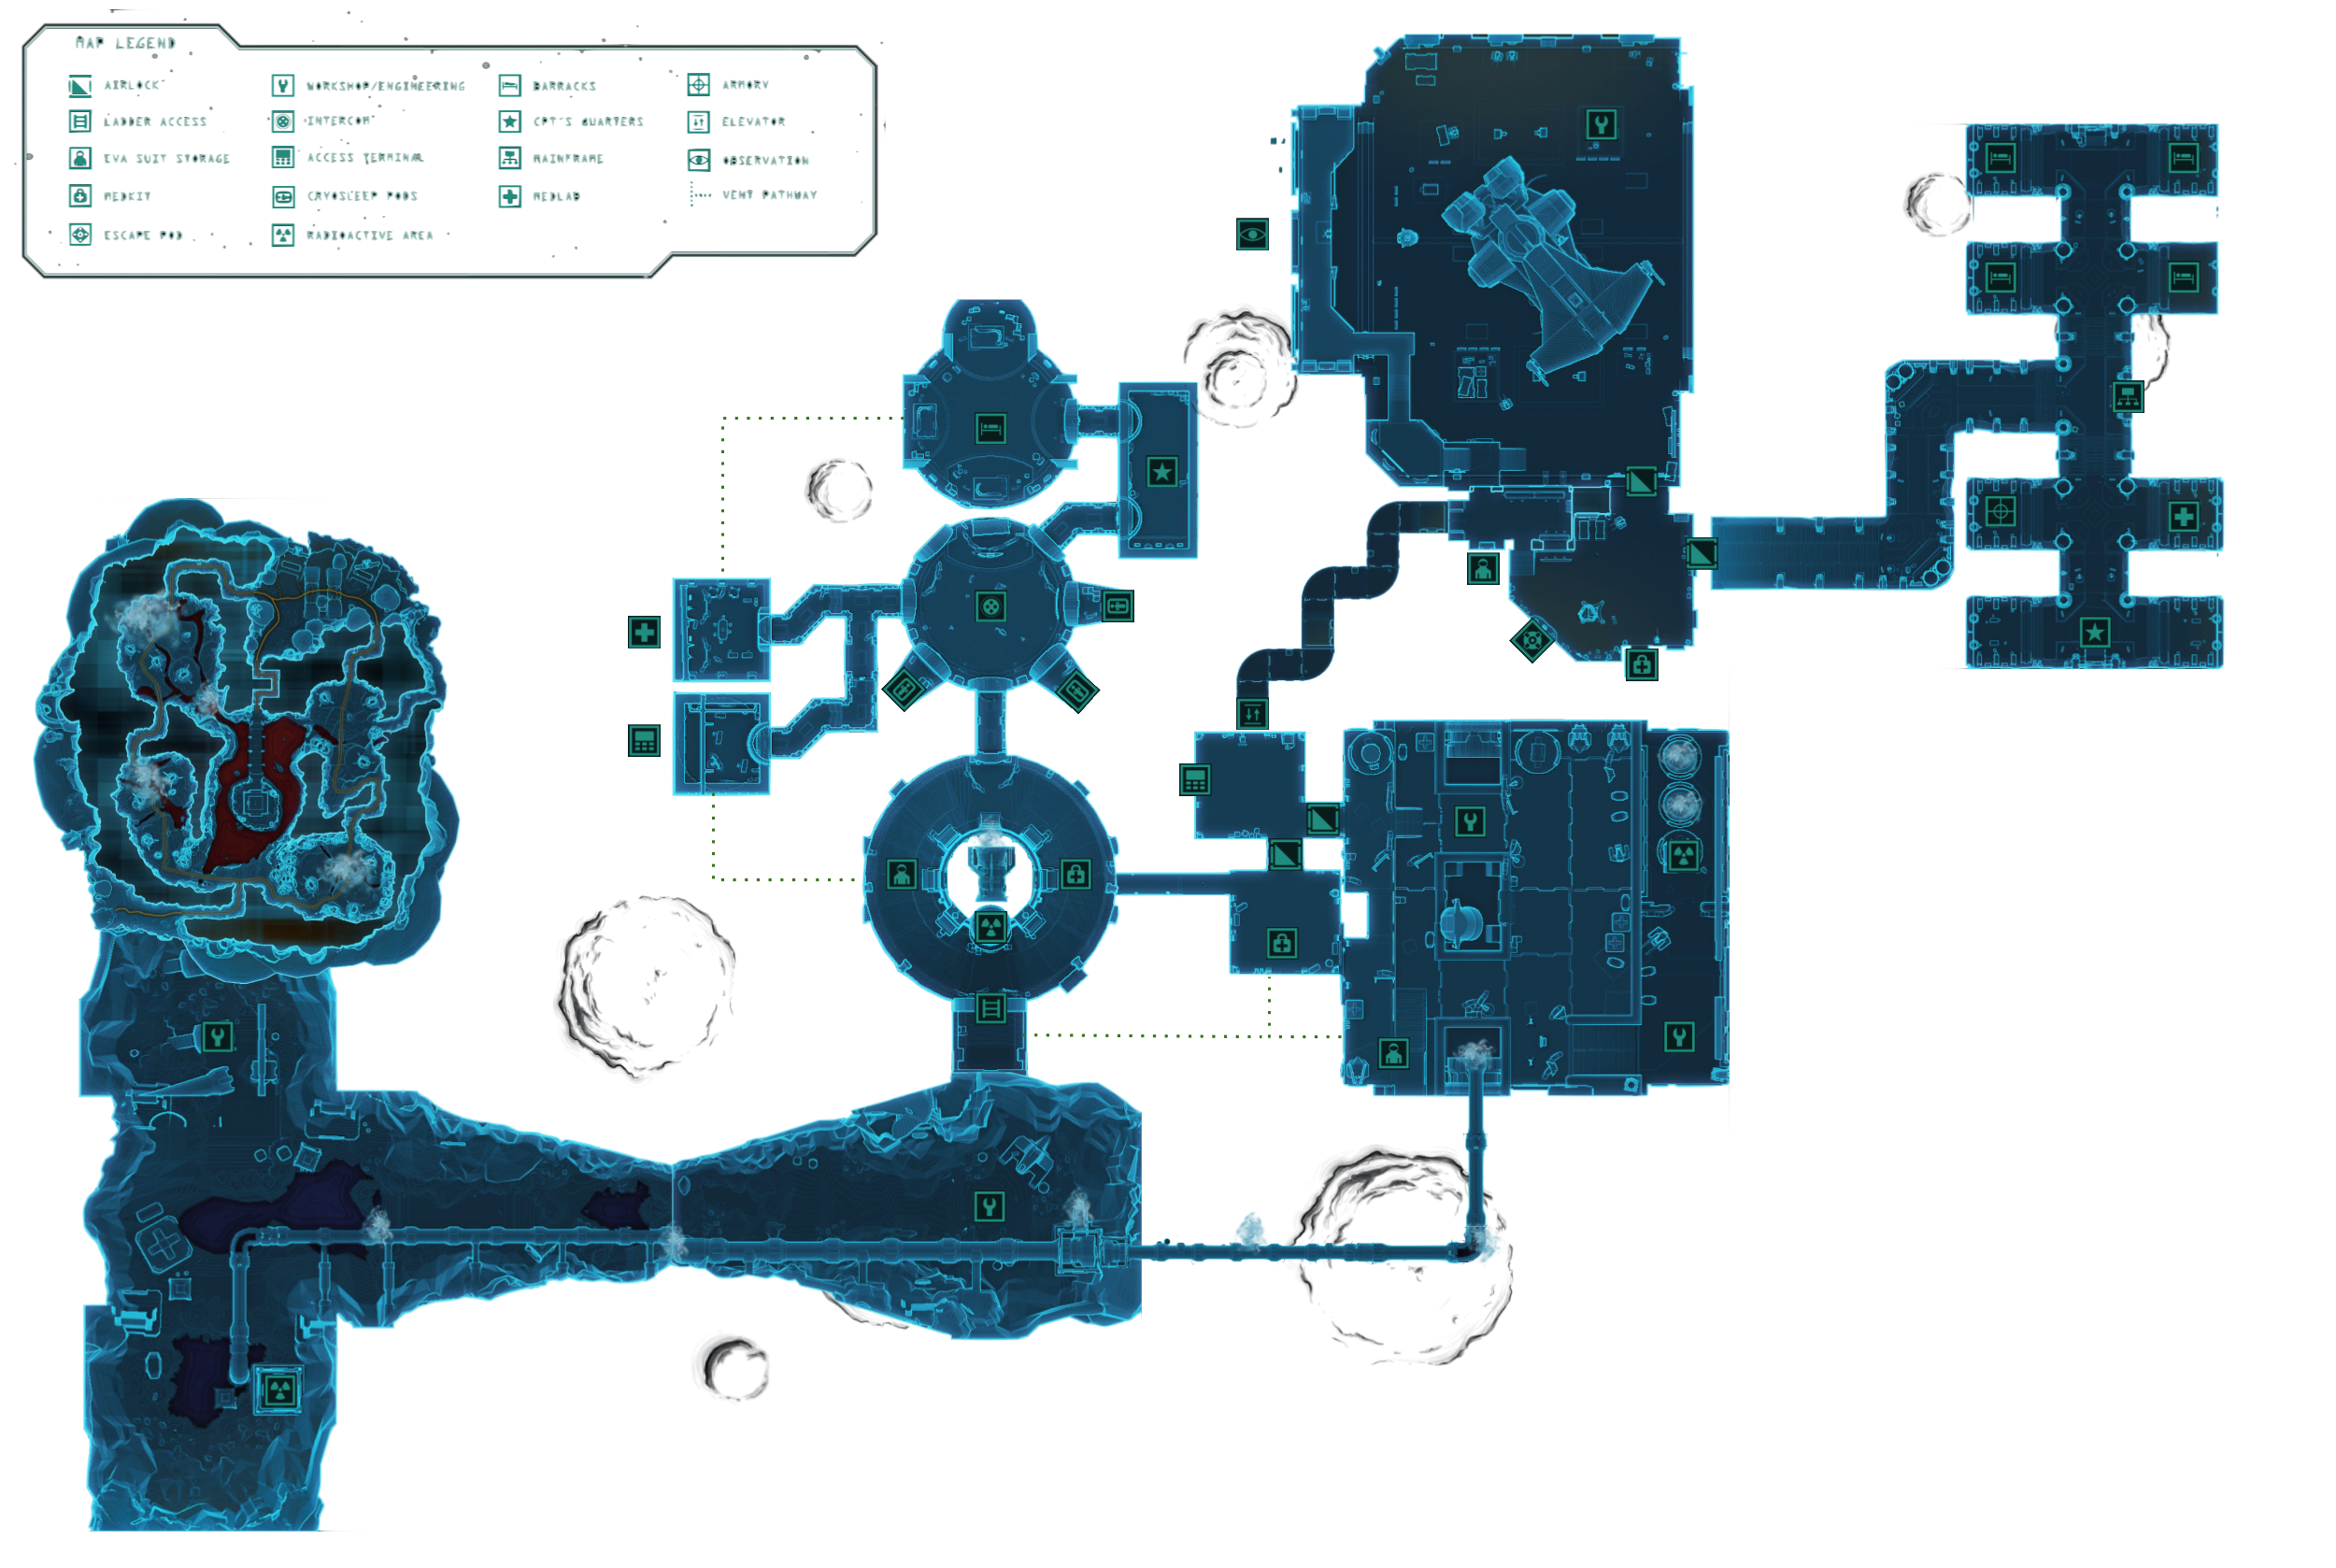
\includegraphics[width=1.05\textwidth]{img/space-refinery-final.png}
    \label{fig:refinery}
\end{sidewaysfigure*}

\newpage
\chapter{Characters}


\section{Prisoners}


Why the prisoners don't just blow up the place? Well, truth to be told most of them are indeed terrorists and they have plans to either escape, gain control of the station as a new rendezvous point, or take revenge on both United Americas or  Weyland-Yutani. Let's just all accept any plausible excuses and have some fun playing RPG. 



\begin{rpg-pcbox}{Andy Myers}{img/andy.png}
    A drug dealer. You have dwarfism and, over the years, you learned how to use this so that you passed unnoticed through marshals and law enforcement. 
\end{rpg-pcbox}

\begin{rpg-commentbox}{}
    Kid

    \textbf{STRENGTH} 4, \textbf{AGILITY} 3, \textbf{WITS} 2, \textbf{EMPATHY} 5

    \textbf{HEALTH}: 4

    \textbf{SKILLS}: Ranged Combat 1, Mobility 1, Piloting 2, Observation 2, Medical Aid 1, Command 3
    
    \textbf{TALENT}: Pull Rank
    
    \textbf{SIGNATURE ITEM}: Jacket patch with WeylandYutani logo    
\end{rpg-commentbox}

\newsect

\medskip \medskip \medskip \medskip \medskip \medskip \medskip \medskip \medskip \medskip \medskip \medskip \medskip \medskip \medskip \medskip \medskip \medskip

\begin{rpg-pcbox}{Fredy Cooperr}{img/fredy.png}
    One of the most fearsome terrorists on anchor point station 2. You fought against corporate greed and blew several Weyland-Yutani installations before arrest. 
\end{rpg-pcbox}

\begin{rpg-commentbox}{}
    Officer

    \textbf{STRENGTH} 4, \textbf{AGILITY} 3, \textbf{WITS} 2, \textbf{EMPATHY} 5

    \textbf{HEALTH}: 4

    \textbf{SKILLS}: Ranged Combat 1, Mobility 1, Piloting 2, Observation 2, Medical Aid 1, Command 3
    
    \textbf{TALENT}: Pull Rank
    
    \textbf{SIGNATURE ITEM}: Jacket patch with WeylandYutani logo    
\end{rpg-commentbox}

\newsect

\begin{rpg-pcbox}{Jone Heson}{img/jone.png}
    You were wrongly accused for a crime you did not commit. You are a hardworking person and you had hopes that Weyland-Yutani lawyers would reach out and save you. Until then, you have to blend in and survive.
\end{rpg-pcbox}

\begin{rpg-commentbox}{}
    roughneck

    \textbf{STRENGTH} 4, \textbf{AGILITY} 3, \textbf{WITS} 2, \textbf{EMPATHY} 5

    \textbf{HEALTH}: 4

    \textbf{SKILLS}: Ranged Combat 1, Mobility 1, Piloting 2, Observation 2, Medical Aid 1, Command 3
    
    \textbf{TALENT}: Pull Rank
    
    \textbf{SIGNATURE ITEM}: Jacket patch with WeylandYutani logo    
\end{rpg-commentbox}

\newsect


\begin{rpg-pcbox}{Ivan Beschastnikh}{img/ivan.png}
    ``dishonorably discharged'' you do not talk about the reason why they threw you in this place either as a punishment worst than death or as a last favor. You are simply ruthless and think that in 3 to 6 months you will be back in the military under some black-ops team.
\end{rpg-pcbox}

\begin{rpg-commentbox}{}
    ex-marine

    \textbf{STRENGTH} 4, \textbf{AGILITY} 3, \textbf{WITS} 2, \textbf{EMPATHY} 5

    \textbf{HEALTH}: 4

    \textbf{SKILLS}: Ranged Combat 1, Mobility 1, Piloting 2, Observation 2, Medical Aid 1, Command 3
    
    \textbf{TALENT}: Pull Rank
    
    \textbf{SIGNATURE ITEM}: Jacket patch with WeylandYutani logo    
\end{rpg-commentbox}

\newsect

\begin{rpg-pcbox}{Hite Chyio}{img/hite.png}
    You were a Yakuza boss. You have blackmail information on several politicians and Weyland-Yutani. Kathia Rison is on her way to get you out of this hell. 
\end{rpg-pcbox}

\begin{rpg-commentbox}{}
    ex-Yakuza

    \textbf{STRENGTH} 4, \textbf{AGILITY} 3, \textbf{WITS} 2, \textbf{EMPATHY} 5

    \textbf{HEALTH}: 4

    \textbf{SKILLS}: Ranged Combat 1, Mobility 1, Piloting 2, Observation 2, Medical Aid 1, Command 3
    
    \textbf{TALENT}: Pull Rank
    
    \textbf{SIGNATURE ITEM}: Jacket patch with WeylandYutani logo    
\end{rpg-commentbox}


\newsect

\medskip \medskip \medskip \medskip \medskip  \medskip \medskip \medskip \medskip \medskip 

\begin{rpg-pcbox}{Henrique Santiago}{img/henrique.png}
    You trafficked people for organs extraction. It suffices to say that your lack any moral restraints.
    Inside the prison, you pulled some favors so that you could smuggle small items. While your new ``business' has been successful, you are paranoid about being caught by a synthetic
\end{rpg-pcbox}

\begin{rpg-commentbox}{}
    Smuggler

    \textbf{STRENGTH} 4, \textbf{AGILITY} 3, \textbf{WITS} 2, \textbf{EMPATHY} 5

    \textbf{HEALTH}: 4

    \textbf{SKILLS}: Ranged Combat 1, Mobility 1, Piloting 2, Observation 2, Medical Aid 1, Command 3
    
    \textbf{TALENT}: Pull Rank
    
    \textbf{SIGNATURE ITEM}: Jacket patch with WeylandYutani logo    
\end{rpg-commentbox}

\newsect

\begin{rpg-pcbox}{Nolan Alder}{img/nolan.png}
    A bio-terrorist. Before being caught, you left a sample of Chemical Agent A0-3959X.91–15 in a hidden stash. You plan to escape and launch a bio attack against anchor point station 2
\end{rpg-pcbox}

\begin{rpg-commentbox}{}
    Scientist

    \textbf{STRENGTH} 4, \textbf{AGILITY} 3, \textbf{WITS} 2, \textbf{EMPATHY} 5

    \textbf{HEALTH}: 4

    \textbf{SKILLS}: Ranged Combat 1, Mobility 1, Piloting 2, Observation 2, Medical Aid 1, Command 3
    
    \textbf{TALENT}: Pull Rank
    
    \textbf{SIGNATURE ITEM}: Jacket patch with WeylandYutani logo    
\end{rpg-commentbox}



\clearpage


\section{Lasalle Bionational crew}

Disguised as Weyland-Yutani annual inspection crew, the Lasalle plans to rescue one of the prisoners who has valuable information against their competitors.




\begin{rpg-pcbox}{Aleki Bowman}{img/bowman.png}
    Chief of security of the Lasalle Bionational crew. You served for many years as a colonial marine, though you noticed that you were a pawn in the corporate/governmental chess match.
\end{rpg-pcbox}

\begin{rpg-commentbox}{}
    mercenary

    \textbf{STRENGTH} 3, \textbf{AGILITY} 5, \textbf{WITS} 2, \textbf{EMPATHY} 3

    \textbf{HEALTH}: 3

    \textbf{SKILLS}: Ranged Combat 2, Mobility 2, Piloting 1, Command 2, Manipulation 1, Combat 1
    
    \textbf{TALENT}: Overkill
    
    \textbf{GEAR}: Armat M41A Pulse Rifle (geo-locked), M3 PERSONNEL ARMOR, dog tag

    \textbf{BUDY}: Tery
    
    \textbf{RIVAL}: Barby
\end{rpg-commentbox}

\newsect

\begin{rpg-pcbox}{Barby Lopez}{img/lopez.png}
    you brought Kathia on her corporate mission though you know the fame of Kohru and had you had the opportunity, you wouldn't think twice about shutting down the place
\end{rpg-pcbox}

\begin{rpg-commentbox}{}
    pilot

    \textbf{STRENGTH} 4, \textbf{AGILITY} 3, \textbf{WITS} 2, \textbf{EMPATHY} 5

    \textbf{HEALTH}: 4

    \textbf{SKILLS}: Ranged Combat 1, Combat 1, Heavy Machinery 1, Mobility 1, Piloting 2, Observation 1, Stamina 1, Manipulation 1, Comtech 1, Survival 1, Command 1
    
    \textbf{TALENT}: Fast Reflexes
    
    \textbf{GEAR}: .357 Magnum Revolver (2 reloads)

    \textbf{BUDY}: Kathia
    
    \textbf{RIVAL}: Aleki
\end{rpg-commentbox}


\newsect

\medskip \medskip \medskip \medskip


\begin{rpg-pcbox}{Kathia Rison}{img/kathia.png}
    On your way to extract Hite from Kohru and get the hell out of this god forsaken place.
    You are arrogant and will always pull your corporate status to get out of messy situations.
\end{rpg-pcbox}

\begin{rpg-commentbox}{}
    Company agent

    \textbf{STRENGTH} 2, \textbf{AGILITY} 3, \textbf{WITS} 4, \textbf{EMPATHY} 4

    \textbf{HEALTH}: 2

    \textbf{SKILLS}: Ranged Combat 2, Mobility 1, Medical Aid 1, Manipulation 3, Observation 2, Comtech 1, Command 3
    
    \textbf{TALENT}: Personal Safety
    
    \textbf{GEAR}: Hairpin

    \textbf{BUDY}: Aleki
    
    \textbf{RIVAL}: Tery
\end{rpg-commentbox}


\newsect

\begin{rpg-pcbox}{Tery Marte}{img/tery.png}
    An activist, you have a hidden camera in your right arm and you falsified paperwork to present yourself as a psychologist. You plan to evaluate the prisoners as an excuse to get first hand data on Kohru and use that for blackmailing or to shut the place down
\end{rpg-pcbox}

\begin{rpg-commentbox}{}
    Roughneck reporter

    \textbf{STRENGTH} 3, \textbf{AGILITY} 3, \textbf{WITS} 4, \textbf{EMPATHY} 4

    \textbf{HEALTH}: 3

    \textbf{SKILLS}: Stamina 2, Survival 1, Comtech 3, Manipulation 2, Medical Aid 2, Mobility 2
    
    \textbf{TALENT}: The long haul
    
    \textbf{GEAR}: Digital Camera

    
    \textbf{BUDY}: Aleki
    
    \textbf{RIVAL}: Kathia
\end{rpg-commentbox}


\clearpage

\subsection{Personal Agendas}

\begin{rpg-commentbox}{Kathia Rison the company agent}
    \begin{enumerate}[label=\textbf{Act \arabic*}, leftmargin=1cm]
        \item Make sure Mageed and the others believe your crew works for Lasalle
        \item Survive
        \item Change the flight plans in the main frame to get you to terrorist space
    \end{enumerate}
    
\end{rpg-commentbox}


\begin{rpg-commentbox}{Tery Marte the reporter}
    \begin{enumerate}[label=\textbf{Act \arabic*}, leftmargin=1cm]
        \item Record prisoner struggles \textbf{requires one mobility and one comtech roll}
        \item Record alien \textbf{requires two slow actions}
        \item Make sure records are released somehow
    \end{enumerate}
\end{rpg-commentbox}



\begin{rpg-commentbox}{Barby Lopez the pilot}
    Change one of the PC agendas by this one. While undercover, the synthetic uses the same attributes as a normal character.

    \begin{enumerate}[label=\textbf{Act \arabic*}, leftmargin=1cm]
        \item Mingle with the crew, making them confess something illegal that happened in the facility
        \item Make the refinery reactor overheat. The station will ultimately explode after T-minus 1 hour
        \item Get back to the ship
    \end{enumerate}
\end{rpg-commentbox}


\begin{rpg-commentbox}{Aleki the mercenary}
    Change one of the PC agendas by this one. While undercover, the synthetic uses the same attributes as a normal character.

    \begin{enumerate}[label=\textbf{Act \arabic*}, leftmargin=1cm]
        \item Assert that no one threatens Kathia
        \item Make sure Hite stays alive
        \item Get heavy weapons in the weapon-locker
    \end{enumerate}
\end{rpg-commentbox}


\clearpage




\section{Kohru crew}


\begin{rpg-pcbox}{Joyce Anderson}{img/joyce.png}
    The chief engineer of the station. This was supposed to be an one-year temporary job. One year turned into two, then into five. You would love to see the place collapse and get a job somewhere safer.
\end{rpg-pcbox}

\begin{rpg-commentbox}{}
    Roughneck

    \textbf{STRENGTH} 4, \textbf{AGILITY} 3, \textbf{WITS} 2, \textbf{EMPATHY} 5

    \textbf{HEALTH}: 4

    \textbf{SKILLS}: Ranged Combat 1, Mobility 1, Piloting 2, Observation 2, Medical Aid 1, Command 3
    
    \textbf{TALENT}: Pull Rank
    
    \textbf{SIGNATURE ITEM}: Jacket patch with WeylandYutani logo    
\end{rpg-commentbox}

\newsect

\begin{rpg-pcbox}{Victor Macbeth}{img/victor.png}
    Chief medic on the station. You live for your job and you actually believe in redemption. You decided to work at this place by choice and all the prisoners seem to understand that. If one person can walk freely in the prison block, that person is you.
\end{rpg-pcbox}

\begin{rpg-commentbox}{}
    Medic

    \textbf{STRENGTH} 4, \textbf{AGILITY} 3, \textbf{WITS} 2, \textbf{EMPATHY} 5

    \textbf{HEALTH}: 4

    \textbf{SKILLS}: Ranged Combat 1, Mobility 1, Piloting 2, Observation 2, Medical Aid 1, Command 3
    
    \textbf{TALENT}: Pull Rank
    
    \textbf{SIGNATURE ITEM}: Jacket patch with WeylandYutani logo    
\end{rpg-commentbox}


\newsect

\medskip \medskip \medskip \medskip \medskip \medskip \medskip \medskip


\begin{rpg-pcbox}{Abdul Mageed}{img/mageed.png}
    A pragmatic. You run the entire station making sure that prisoners don't kill each other (more than the necessary to blow steam off). You turn a blind-eye to people wrongly accused thinking that the few false positives justify all the greater good.
\end{rpg-pcbox}

\begin{rpg-commentbox}{}
    Colonial marshal

    \textbf{STRENGTH} 4, \textbf{AGILITY} 3, \textbf{WITS} 2, \textbf{EMPATHY} 5

    \textbf{HEALTH}: 4

    \textbf{SKILLS}: Ranged Combat 1, Mobility 1, Piloting 2, Observation 2, Medical Aid 1, Command 3
    
    \textbf{TALENT}: Pull Rank
    
    \textbf{SIGNATURE ITEM}: Jacket patch with WeylandYutani logo    
\end{rpg-commentbox}


\newsect

\begin{rpg-pcbox}{Mik Elson}{img/mik.png}
    Chief of security. You hate your job. You are trapped in this living hell with some of the worst scum of the sector. You would sacrifice each and every one for your personal survival.
\end{rpg-pcbox}

\begin{rpg-commentbox}{}
    Marine

    \textbf{STRENGTH} 4, \textbf{AGILITY} 3, \textbf{WITS} 2, \textbf{EMPATHY} 5

    \textbf{HEALTH}: 4

    \textbf{SKILLS}: Ranged Combat 1, Mobility 1, Piloting 2, Observation 2, Medical Aid 1, Command 3
    
    \textbf{TALENT}: Pull Rank
    
    \textbf{SIGNATURE ITEM}: Jacket patch with WeylandYutani logo    
\end{rpg-commentbox}

\newsect



% \begin{rpg-commentbox}{Joyce Ardson}
%     roughneck: 
% \end{rpg-commentbox}

% \begin{rpg-commentbox}{}
%     medic: 
% \end{rpg-commentbox}

% \begin{rpg-commentbox}{}
%     marine: 
% \end{rpg-commentbox}

% \begin{rpg-commentbox}{Abdul Mageed}
%     : 
% \end{rpg-commentbox}




% \section{NPCs}

% In case you need sidekicks.

% \begin{rpg-commentbox}{random prisoners}
%     \begin{itemize}
%         \item Mito Yoran
%         \item Edzuk Shiro
%         \item Bomba Andres
%         \item Edison Harcrow
%         \item Brom Tower
%         \item Delphine Ryant
%     \end{itemize}

% \end{rpg-commentbox}


% \begin{rpg-commentbox}{Random staff}
%     \begin{itemize}
%         \item Aleve Miroste
%         \item Psycho Dante
%         \item West Nylund
%         \item Jocasta Belmont
%         \item Geneva Macbeth
%         \item Monte Jann
%         \item Hawthorne Thoran
%         \item Harrison Woldt
%     \end{itemize}

% \end{rpg-commentbox}

% \newsect

\chapter{Act I}



\begin{rpg-commentbox}{}

    Corporate people arrive at the station and \pc{Kathia} wants to bring a \pc{PC} back to Lasalle Bionational territory. She speaks with the station marshal Abdul Mageed and is allowed to take the elevator down to refinery levels where she can talk with the prisoner.

    Either all or part of her crew go down with her to ensure her security (Mik and Victor) or to play some role in the extraction (Tery and Aleki). 
    
\end{rpg-commentbox}


% \medskip
% \begin{rpg-commentbox}{Lasalle Objectives}
% If you plan to run the adventure using the crew make sure that either no one follows Kathia to prison OR that players are equally divided between station and prison levels.

% \begin{itemize}
%     \item Potential introductions

%     \item Negotiation between the Lasalle and Kohru crews. \textbf{manipulation} \textbf{command}
% \end{itemize}
% \end{rpg-commentbox}



\medskip
\begin{rpg-commentbox}{Prisoner Objectives}
For the prisoners, keep them busy dividing them either at the mining area or the refinery area. Some events to serve as ice breakers:

\begin{itemize}
    \item There is a solar glass panel that is not protecting against ultraviolet radiation in the refinery. Part of the crew should fix that. An entire shift can fix a small portion of the panel but not everything. This will have a role later on. \textbf{heavy machinery}

    \item Rumors spread that there is a synthetic amongst the prisoners and people plot how to rule out who is the synthetic to feed misinformation to it \textbf{observation}

    \item A potential murder attempt among the prisoners \textbf{close combat}

    \item Bartering among prisoners \textbf{manipulation}
\end{itemize}
\end{rpg-commentbox}


\newsect

\section{Station Lockdown}



\begin{rpg-commentbox}{}
    
    Within some of the lithium ore, there are parasite spores created by the engineers. When the ore is heat and pulverized in the refinery section, a small parcel of the parasites spread through the station ducts. Two will make their way to hosts in the refinery section while a third one will infect someone at the crew quarters. 
    
    The Kohru computer system, \textbf{Dexter}, warns about environmental hazard contamination and puts the station in lockdown. Increase stress level by 1
\end{rpg-commentbox}    


\medskip
\begin{rpg-commentbox}{Notes for potential escape plans}
\begin{itemize}
    \item The only person with a corporate key card is at the prison (Kathia). The card is necessary to turn the engines of the Lasalle Bionational ship back online if anyone plans to escape. The keycard is \textbf{either} in Kathia's possession or locked under some biometric safe with instructions to corrupt the card if anyone tries to crack it open. 

    \item It's also necessary to open the landing hatch. Potential solutions involve using the sulfuric acid in the refinery or blowing the thing open. Either option will take the air out of the refinery and if done before the keycard is retrieved, that will put all future events on a timer. I advise to run for air supply periodically.
\end{itemize}
\end{rpg-commentbox}


% \begin{quotation}
% \begin{small}
% \textit{}

% \textit{}    
% \end{small}    
% \end{quotation}
    


\newsect

\newpage

\section{Escape plan}


\begin{rpg-commentbox}{}
    Lock-down won't let the elevator between the levels work until environment measurements are back to standard levels.
    
    
    The prisoners can check air filters at several locations to make sure the station's system is not just malfunctioning. In fact this is not the first time that something similar has happened. At some point, one of the prisioners will be brought back to medical where he start having convulsions...

\end{rpg-commentbox}

\begin{rpg-commentbox}{The Alien}
    This is also a good place for foreshadowing. Describe via radio communication some prisoners saying that some strange ore was found in the pulverizer or things that allude to an extra presence in the prison ward.
 \end{rpg-commentbox}




\begin{rpg-commentbox}{Infection stages}
    \begin{enumerate}
        \item convulsions and med bay
        \item splitting blood and more seizures
        \item host's death
    \end{enumerate}

    At this point, players are probably expecting the creature to burst out of the host. However, it won't happen and the spore will keep growing and merging its DNA with the hosts. Let them discuss and imagine whether this was a heart attack or something else. All initial attempts will point to a normal disease and equipment for an autopsy is only available at the upper level.  \textbf{medical aid}

\end{rpg-commentbox}





\newsect

\section{Heated discussion}


\begin{rpg-commentbox}{}
    
    Draw the players' attention somewhere else other than the dead body. If one player decides to stay behind and watch for the corpse, this may have several consequences in the game and a potential early death.
    
    -- A potential event is a discussion in the intercon between Kathia and Mageed, where Kathia desperately tries to convince him of escorting her out of the prison ward \textbf{manipulation}
    
    -- Tery can also reveal his hidden camera and say that he has footage that could ruin the Marshal's career

\end{rpg-commentbox}

\newsect



\begin{rpg-commentbox}{Fresh meat in the prison block}
    
    Negotiation to escape the prison ward is not successful. When players get back to the dead body's location, it is missing. Increase stress level by 1.
    
    There is a trail of blood leading into either the refinery direction or the mines. If one of the players stayed behind they witness:
    
    \textit{
    ``The alien is parasitic. It is still feeding from the host and using its motor system while it grows stronger. At this stage, players can see a protuberance in the person's back, exposed insect like tendrils ripping through the flesh, broken bones, and four long and thin spider-like appendages sprouting from the the host's back. The creature uses these sharp appendages to attack and kill potential threats or to infect new victims''.
    } 

    \medskip
    
    
    Roll a combat scene between any players that stayed behind and the creature. \textbf{Alien is at stage I (host attached)}
    
    If attacked and threatened, the creature can detach from the host and escape thorough an air duct. It will eventually find a new host in the mines.
    
    

\end{rpg-commentbox}    


\begin{rpg-commentbox}{Corporate security comes first}
    Kathia will persuade the prisoners to safeguard her and take her out of the station. Any prisoners protecting her will receive new identities in Lasalle Bionational controlled space.
\end{rpg-commentbox}
    


\begin{rpg-commentbox}{End of Act}
    \textbf{Act 1 ends when prisoners notice the missing body OR fight the stage I alien.}
 \end{rpg-commentbox}
\chapter{Act II}




\section{Where the hell is the body?}


\begin{rpg-commentbox}{The Alien}
   The creature controls the host to seek a dark and quiet place where it can grow stronger eventually reaching stage II.

    On its path, it will infect two more prisoners making a larva exo-parasite grow on the host's stomach. 
    The larva are in stealth mode and they need to infect a new host to reach stage II.

    \medskip

    If the PCs had killed the first alien, just have some other prisoners infected and describe gore bodies as they walk through the refinery
\end{rpg-commentbox}


\newsect

\section{Escape plan}


\begin{rpg-commentbox}{Protect Kathia}
    Ideally, Kathia has left her corporate card in a biometric safe, so her protection is paramount to any escape plan.

    Mageed contacts prisoners via intercom and says that the crew is working on a escape plan. They will use Kathia's ship and for that, they need to bypass the lockdown.
    Prisoners are asked to gather enough mining explosives and bring them to the reactor core at the refinery. A handful of explosives can damage the reactor and cut power in the station, that will deactivate the lockdown. However, prisoners will need EVA suits as the air in the station will soon deplenish.
 \end{rpg-commentbox}


 \begin{rpg-commentbox}{Grab Explosives at the mine}
    Depending how players go fetch the mining explosives, they will face the alien fully morphed to stage 2. \textbf{Alien has stats of a Xenomorph stalker}

    Run a stealth mode scene moving some of the players through the mines. \textbf{mobility} vs \textbf{observation}
 \end{rpg-commentbox}


 
 \begin{rpg-commentbox}{Bring explosives to reactor}
    At this point in time, if one of the larva is still alive and the PCs did not encounter it, people will hear agonizing screams as the larva infects a new host. 

    Something cool for this one is to let the host have a welding torch. The alien won't use it but it hangs in a loosely held bandoleer making a lot of noise while the exo-parasite walks the refinery. This can make for some interesting scenes as for example, players setting the explosives in the reactor core while listening to the crackling sound of metal against the crate floor.

    Players must hack the reactor door \textbf{comtech}, put the explosives and set a controlled explosion \textbf{??} Failures might bring nice complications
 \end{rpg-commentbox}

 \begin{rpg-commentbox}{Load cargo elevator with sulfuric acid}
    Needed to crack safe open without corrupting the corporate card

    Players must use crane to pick acid containers \textbf{heavy machinery}
 \end{rpg-commentbox}


 \begin{rpg-commentbox}{Other option}
   Other option is to switch the strategy, use sulfuric acid to open a pathway to the upper level and the mines for opening the hangar hatch.
\end{rpg-commentbox}

 \newsect

 \section{What is happening upstairs?}
 
\begin{rpg-commentbox}{We've got a situation here}
   From time to time Mageed gets in the intercom and give instructions. At some point, let him say hang-on, we got a situation here. All communications after this only return hiss static. Increase stress level by 1.
\end{rpg-commentbox}
\chapter{Act III}
\lipsum[1] % filler text
\chapter{Appendix}

  


\begin{figure*}
    \centering
    
\includegraphics[width=.8\textwidth]{img/stage-III-bg.png}
    \caption*{The Exo-Alien}
\end{figure*}


\clearpage

\section{Exo-parasite}

\begin{rpg-commentbox}{Exo-parasite}
    The parasite is a scorpion like creature with four strong legs a tail ending on a powerful sting and a huge maw under its bely. The maw and stings on the creature's legs have powerful neurotoxin able to jeopardize a host's motor abilities. The host is lethargic, yet still alive and in the moments it is not under the effects of the toxin, it can feel the creature tentacles moving though your organs and slowly feeding from your corpse. 
\end{rpg-commentbox}    


\begin{rpg-commentbox}{}

    \centering{\textbf{Stats}}

    \par\noindent\rule{\textwidth}{0.4pt}

    \textbf{SPEED} 2

    \textbf{HEALTH}: 2

    \textbf{SKILLS}: Mobility 8, Observation 8
    
    \textbf{ARMOR}: 2 (0 vs fire)
    
    \textbf{ACID SPLASH}: 4

    \par\noindent\rule{\textwidth}{0.4pt}

    \begin{small}
    \begin{enumerate}
        \item SKITTERING MENACE The parasite has chosen its host and they know it is coming for
        them! It skitters forward, single-minded and horrifyingly spider-like. The victim suffers +1
        STRESS LEVEL and must make an immediate Panic Roll.
        \item same as above
        
        \par\noindent\rule{.9\textwidth}{0.4pt}

        \item TAIL LASH The little monster comes for its target, lashing out with its wicked tail. It attacks
        with five Base Dice, Damage 1.

        \par\noindent\rule{.9\textwidth}{0.4pt}

        \item TAIL GRAPPLE: The parasite leaps and catches its victim from behind, its tail whipping
        violently. Roll a D6:
            1–2: The target’s legs are caught and they fall prone — make a Panic Roll.
            
            3–4: The victim’s arms get hopelessly tangled in the beast’s tail — they cannot use any held items and must make a Panic Roll.
            
            5–6: The parasite wraps its tail around the target’s neck, choking them — they suffer the effects of DROWNING and must make a Panic Roll. 

        \par\noindent\rule{.9\textwidth}{0.4pt}

        \item SPINE GRAPPLE The parasite leaps at its victim. Make an opposed roll with six Base Dice
        against the target’s CLOSE COMBAT skill (not counting as an action for the victim):
            If the parasite wins, the target will suffer THE FINAL EMBRACE (below) on the parasite's next initiative.

            If the victim wins they throw the beast to the floor, but it’s not finished with them
        yet and attacks the same target again on its next initiative. 

        \par\noindent\rule{.9\textwidth}{0.4pt}

        \item THE FINAL EMBRACE The parasite gets to its victim, its acid making short work of any armor or respirator in the way. Roll for the attack with six Base Dice. If it gets one or more, the poor victim is hugged and immediately Broken.
    \end{enumerate}
    \end{small}

\end{rpg-commentbox}

\begin{rpg-commentbox}{Host}
    While attached to a host, the creature seeks a quiet place where it can fully merge its DNA with the host, dropping the empty shell and taking full control of the host. If attacked, first deduce any damage from the host. If the host dies, the creature detaches and it will try to escape or attach itself to a new host.
    While attached, substitute 5s and 6s with:

    \par\noindent\rule{.9\textwidth}{0.4pt}

    ALL-OUT ATTACK: The exo-parasite launches into a wild attack, throwing every one of its sting legs at its victim. It attacks with eight Base Dice, Damage 1.

\end{rpg-commentbox} 


\begin{figure}
    \centering
    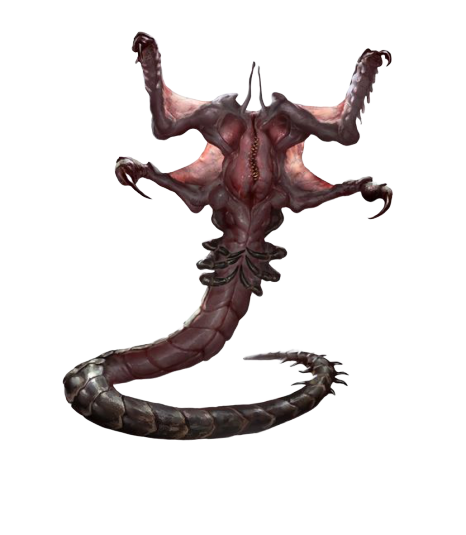
\includegraphics[width=.45\textwidth]{img/stage-I-bg.png}
    \label{fig:stage-1}
    \caption*{Stage I - Exo-parasite}
\end{figure}


\clearpage

\section{Exo-host}

\begin{rpg-commentbox}{Exo-host}
    The parasite has taken full control of its host. Its spider like legs have doubled in length now serving as powerful defensive appendages able to impale any human being. At this stage, it starts producing spores that it can inject into new hosts through its leg stings. 
\end{rpg-commentbox}    


\begin{rpg-commentbox}{}

    \centering{\textbf{Stats}}

    \par\noindent\rule{\textwidth}{0.4pt}

    \textbf{SPEED} 2

    \textbf{HEALTH}: 6

    \textbf{SKILLS}: Mobility 8, Observation 6
    
    \textbf{ARMOR}: 10 (5 vs fire)
    
    \textbf{ACID SPLASH}: 8

    \par\noindent\rule{\textwidth}{0.4pt}

    \begin{small}
    \begin{enumerate}
        \item HYPNOTIZING GAZE: The decomposing eyes of the host stare deeply into the soul of its
        victim. The victim is mesmerized by the dread of such a beast. They stand in awe of
        what nature, or god, or the devil has created, get +1 STRESS LEVEL and must make an immediate Panic Roll.

        \par\noindent\rule{.9\textwidth}{0.4pt}
        
        \item  ASSESSING THE THREAT: The host pauses, hissing quietly but all the more threatening
        for that. It looks like it’s thinking, 
        or maybe giving silent orders to unseen companions. Everyone within MEDIUM range gets +1 STRESS LEVEL.

        \par\noindent\rule{.9\textwidth}{0.4pt}

        \item PLAYING WITH ITS PREY: The host attacks, but not to kill. The target is knocked to the ground
        and drops all hand-held items, but otherwise takes no damage. The host stands over
        them, taunting its prey to run so the game can go on. The victim gets +1 STRESS LEVEL and
        must make an immediate Panic Roll.
        
        \par\noindent\rule{.9\textwidth}{0.4pt}

        \item ALL-OUT ATTACK: The host launches into a wild attack, throwing every one of its sting legs at its victim. It attacks with ten Base Dice, Damage 1. If the victim takes damage, it is infected with a disease with Virulence 6.

        \par\noindent\rule{.9\textwidth}{0.4pt}

        \item READY TO KILL: The host grabs its victim, its parasite stings poised to strike. Roll for the
        attack with ten Base Dice. If it hits, the victim counts as grabbed (see page 93) and needs to
        make an opposed CLOSE COMBAT roll against ten Base Dice to break loose. The victim and all
        friendly characters in the same zone must make Panic Rolls. Unless the victim breaks free,
        the host will use a STINGER TAIL attack against them on its next initiative.

        \par\noindent\rule{.9\textwidth}{0.4pt}


        \item STINGER TAIL: The host's deadly tail leans out,
        gnashing in anticipation before snapping forwards. The attack has a strength of nine Base
        Dice, Damage 2. If it causes any damage it automatically inflicts critical injury \#64, killing
        the victim in one dreadful blow. 
    \end{enumerate}
    \end{small}

\end{rpg-commentbox}

\begin{figure}
    \centering
    
\includegraphics[width=.45\textwidth]{img/stage-II-bg.png}
    \label{fig:stage-2}
    \caption*{Stage II - Exo-host}
\end{figure}

\clearpage

\section{Exo-alien}


\begin{rpg-commentbox}{Exo-alien}
    The decomposing body of the host is transformed into a liquid cocoon. The parasite uses the host's DNA to fully morph into a powerful insect like alien.  The tendrils on its belly carry spores and the exo-alien playfully leave some of its victims alive so it can reproduce. In the lack of victims, its tendrils touches any possible surface making sure that future parasites will infect whoever dares to explore the den of the beast.

\end{rpg-commentbox}    


\begin{rpg-commentbox}{}

    \centering{\textbf{Stats}}

    \par\noindent\rule{\textwidth}{0.4pt}

    \textbf{SPEED} 2

    \textbf{HEALTH}: 8

    \textbf{SKILLS}: Mobility 5, Observation 8
    
    \textbf{ARMOR}: 10 (5 vs fire)
    
    \textbf{ACID SPLASH}: 8

    \par\noindent\rule{\textwidth}{0.4pt}

    \begin{small}
    \begin{enumerate}
        \item ASSESSING THE THREAT: The exo-Alien pauses, hissing quietly but all the more threatening
        for that. It looks like it’s thinking, 
        or maybe giving silent orders to unseen companions. Everyone within MEDIUM range gets +1 STRESS LEVEL.

        \par\noindent\rule{.9\textwidth}{0.4pt}
        
        \item  ALL-OUT ATTACK: The exo-Alien launches into a wild attack, throwing every one of its tendrils at its victim. It attacks with ten Base Dice, Damage 2. If the victim takes damage, it is infected with a disease with Virulence 6.

        \par\noindent\rule{.9\textwidth}{0.4pt}

        \item BEASTLY BITE: The exo-Alien takes a huge bite from its victim. The attack is rolled with ten
        Base Dice, Damage 1. If the attack causes any damage, it inflicts critical injury \#61 even if
        the victim isn’t Broken, triggering a Panic Roll.
        
        \par\noindent\rule{.9\textwidth}{0.4pt}

        \item CRUSHING BLOW: The exo-Alien brings its entire weight down on the poor victim, who must
        make a MOBILITY roll at –2 (no action) or be crushed, immediately suffering three critical
        injuries (roll three times on the critical injury table and apply all three results, regardless of
        whether or not the victim is Broken). The victim is knocked to the ground and must make
        an immediate Panic Roll

        \par\noindent\rule{.9\textwidth}{0.4pt}

        \item TAIL SPIKE: The tail impales the victim with terrible force. Roll for the attack using ten Base
        Dice (fourteen for a Queen), Damage 1. The attack is armor piercing. If the attack causes
        any damage it automatically triggers critical injury \#66, killing them outright

        \par\noindent\rule{.9\textwidth}{0.4pt}


        \item BELLY TENDRILS: The exo-Alien belly tendrils lash out. The attack uses
        ten Base Dice, Damage 2. If it causes any damage the victim immediately suffers critical
        injury \#64, killing them in one dreadful blow.
    \end{enumerate}
    \end{small}

\end{rpg-commentbox}


\begin{figure}
    \centering
    
\includegraphics[width=.6\textwidth]{img/stage-III-bg.png}
    \label{fig:stage-3}
    \caption*{Stage III - Exo-alien}
\end{figure}


\section{Exo-Spore}

\begin{rpg-commentbox}{Exo-spore}
    Released by the exo-alien the spore can survive the test of time, below-zero temperatures, and even high-temperatures. If an exo-alien dies of age or from starvation its carapace makes a cocoon that, when under crush pressure, will explode and release spores in a wide area. This is basically what happened in the refinery. A exo-cocoon fossilized within the lithium ore.
\end{rpg-commentbox}

\clearpage


\section{Thanks}

\begin{rpg-commentbox}{Special thanks to the r/alienrpg community}
    
    \begin{enumerate}
        \item u/A\_Veidt
        \item u/seasparrow32
        \item u/UserNameNotSure
        \item u/shmigglyworgenville
        \item u/\_ArthurDallas\_
    \end{enumerate}
\end{rpg-commentbox} 

\section{Credits}

\begin{rpg-warnbox}{TODO}
    Credit artists
\end{rpg-warnbox}



% End document
\end{document}
